\documentclass[aps,prb,reprint,showpacs,floatfix,superscriptaddress, onecolumn, nofootinbib, 10pt]{revtex4-2}

\usepackage{amsmath,amsthm,amssymb}
\usepackage{graphicx}% Include figure files
\usepackage{dcolumn}% Align table columns on decimal point
\usepackage{bm}% bold math
\usepackage{color}
\usepackage{epsfig}
\usepackage{multirow}
\usepackage{mathrsfs}
\usepackage{hyperref}
\usepackage{cleveref}
\usepackage{epstopdf}
\usepackage{subfigure}
\usepackage{autobreak}
\usepackage{todonotes}
\usepackage{physics}
\usepackage{bbm}
\usepackage[normalem]{ulem}
\usepackage[margin=0.5cm]{geometry}

\usepackage[absolute,overlay]{textpos}

\newcommand{\response}[1]{{\color{black}#1}} % for authors' response
\newcommand{\comment}[1]{{\color{blue}#1}} % for referee's comment

\newcommand{\red}[1]{{\color{red}#1}} % comments during writing
\newcommand{\figref}[1]{FIG.~\ref{#1}}

\renewcommand{\baselinestretch}{1.2}


\begin{document}
\preprint{Preprint}

\title{Response to Referee Comments for Manuscript NJP-117075}
\author{Mahbub Rahaman, Akitada Sakurai, Analabha Roy}
\date{\today}

\maketitle

\vspace{1em}

\noindent \textbf{Response to the Referee: 2's comment}
\begin{enumerate}
	\item {\bf Major Comments}
	\begin{enumerate}
		\item The referee comments on, \comment{``System size dependence: The manuscript presents insightful results for a system size
				of N=8; however, a crucial aspect remains unexplored – the dependence of the
				findings on the system size. How do the observed dynamics and stability vary with an
				increase in system size?"}\\
		
		\response{
			We appreciate the referee's comment. In response, we have conducted further investigations on the formation and stability of quantum chimera-like order for system sizes larger than N=8. In the revised manuscript, we have included figure 9, which shows the plot of regional magnetization ($M^z_A$) and illustrates the occurrence of melting in the DTC phase \red{along with beats present in $M^Z_A$ plot}. We have considered a range of system sizes, N=4,6,8,10 and calculated the numerical values of $M^z_A$ at the DTC/DL point \red{(first root of $\mathcal{J}_0(4h/\omega)$)}. We have also obtained the corresponding Fast Fourier Transforms (FFT) for each $\beta$ value and spin coupling strength. From the FFT data, we have calculated the beat frequency $\delta \Omega_B$ \cite{Liu2023,CHANDRA2024129552}  and plotted it in \figref{Fig:beatsfft}. We have observed that the frequency of beats decreases as the system size N increases, indicating an enhancement in the stability of the DTC-DMBL chimera-like order. In the thermodynamic limit, as N approaches infinity, the beat frequency disappears, indicating a fully stable chimera-like order. We have added a section titled ``4.3. System size-dependent stability in chimera-like order" on page 19 in the revised manuscript to describe this relationship between system size and stability.


			\begin{figure}[h!]
				\begin{center}
					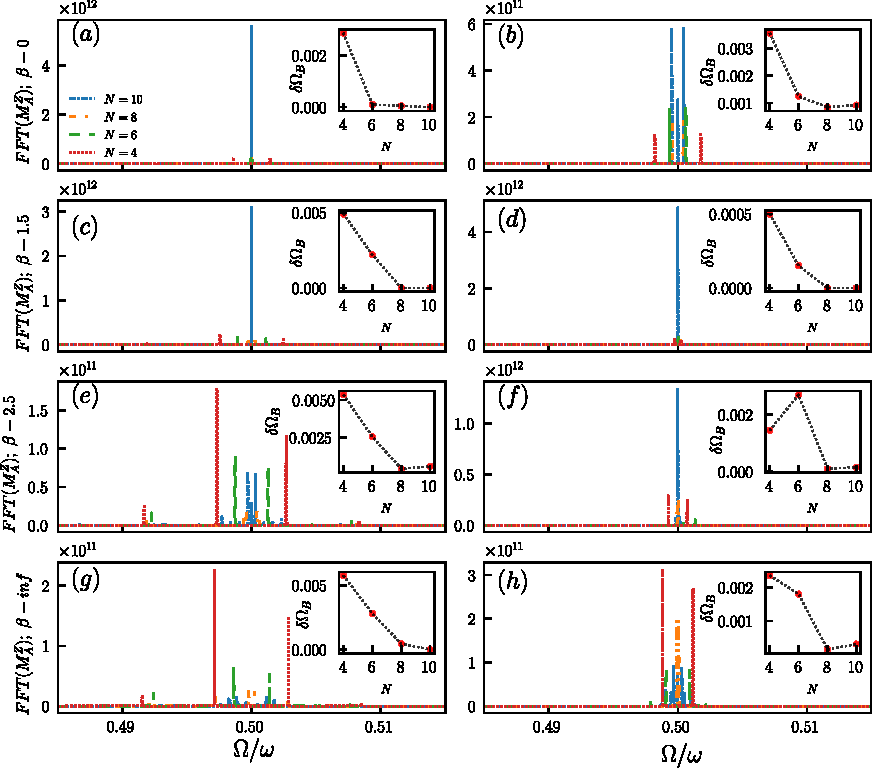
\includegraphics[width=10cm]{./figs/figure12.pdf}
				\end{center}
				\caption{FFT of regional magnetization $M^z_A$ for $8\times10^4$T and spin interaction ranges ($\beta = 0,1.5,2.5, \infty[inf]$) at panels from top to bottom. The left and right panels show weak and strong spin coupling respectively. With constant $\omega = 20$ and time period $T= 2\pi/\omega$, the drive parameters are at the CDT/DL point. Each panel's inset shows the beat frequency ($\delta\Omega_B$) for various system sizes N.
				}
				\label{Fig:beatsfft}
			\end{figure}
		}
	
		\item The referee comments on, \comment{``Influence of rotational error $\epsilon_B$: The manuscript effectively investigates the
			impact of $\epsilon_A$={0.03,0.05,0.1} on the chimera states, leaving the role of $\epsilon_B$, set to 0.9, less discussed. How does varying $\epsilon_B$ impact the chimera
			states?"}\\
		
		\response{We appreciate the referee's interest in this issue. We have conducted further investigations to explore the influence of spin rotation errors, specifically $\epsilon_B$, on the stability of the DTC-DMBL chimera-like order. In the revised manuscript, we have included Figure 7 on page 14, which presents the numerical calculation of the local magnetization $\expval{\hat{S}_z}$ for different $\beta$ values and spin coupling strengths. We have observed that as $\epsilon_B$ decreases, the stability of the DMBL phase in region B decreases, which directly affects the stability of the DTC phase in region A. Additionally, we have examined the regional magnetization $M^z_A$ and $M^z_B$ at the CDT/DL point for various values of $\epsilon_A$ and $\epsilon_B$, as shown in Figure 8 on page 16. We found that the stability of the DTC-DMBL chimera-like order is highest when $\epsilon_A$ approaches 0 and $\epsilon_B$ approaches to 1.0. When $\epsilon_B$ gradually falls below 0.9 and $\epsilon_A$ is kept constant at 0.03, both regions undergoes gradual transition into a melting DTC phase. We have provided a comprehensive discussion on these findings in Section 3 on page 12 para 3 and Section 5.1 on page 15.}
	
		\item The referee comments on, \comment{``\underline{Higher root of Bessel function and stability of chimera states:}"}\\
		\begin{enumerate}
			\item \comment{``The paper introduces a higher root of the Bessel function without explicitly justifying its significance. The importance of this higher root and its relevance to the stability
				of chimera states need clarification. How does the selection of a higher root impact the system's behavior, and why is it crucial for the observed dynamics?"}\\
			
			\response{We appreciate the referee for bringing this issue to our attention. In order to achieve DMBL in the $T_2$ cycle, the ratio of the drive parameter ($h,\omega$) can be \textit{any} one of the roots of the Bessel function $\mathcal{J}_0\left(\frac{4h}{\omega}\right)$.  Our numerical simulations chose the first root by default. Nonetheless, we had to choose a higher root in some simulations for technical reasons. The fact that any root will do can be seen in a comparison below in \figref{Fig:rootissue}. For consistency, we have updated figures 4 and 9 in the revised manuscript for simulations at the first root only.

			\begin{figure}[h!]
				\begin{center}
					\hspace{2cm}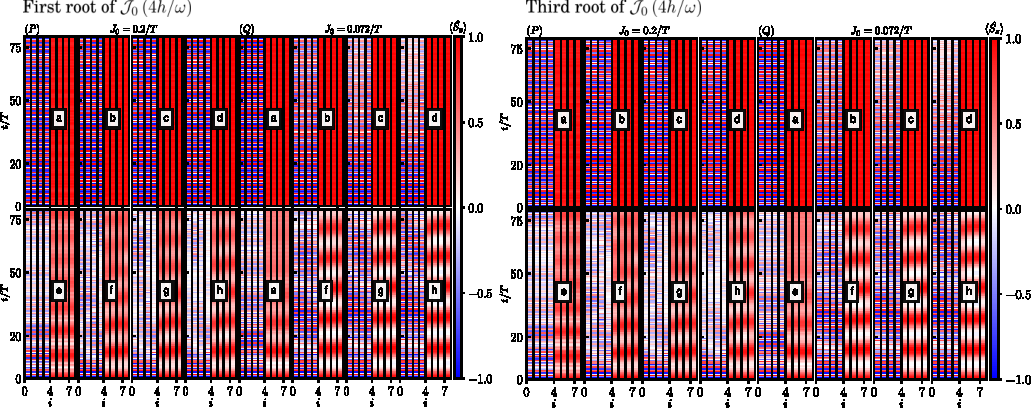
\includegraphics[width=18cm]{./figs/root_comparision.pdf}
				\end{center}
				\caption{The top left panel shows the local magnetization for different $\beta$ at the first root of $\mathcal{J}_0(4h/\omega)$ for $N=8$ up to 80T. In the top right panel shows the local magnetization at the third root of $\mathcal{J}_0(4h/\omega)$ for the same parameters. The bottom panels denote points other than root of $\mathcal{J}_0(4h/\omega)$. The drive frequency is fixed at $\omega=20$ and the drive amplitude is set at the corresponding $\mathcal{J}_0(4h/\omega)$. The temporal variation of $\expval{\hat{S}_z}$ is found to be the same in both panels.}
				\label{Fig:rootissue}
			\end{figure}
		}
			\item \comment{``Moreover, the statement “The stability of the chimera order diminishes even if there is a minor deviation from the CDT/DL point” (page 15, lines 43-44) implies that chimera states might not be stable under slight deviations from the CDT/DL point. This raises a critical question regarding the practical implementation of creating chimera states in experiments. To address this, it would be valuable for the paper to explore potential techniques or strategies aimed at stabilizing the DMBL part of the chain. Elaborating on practical considerations and potential solutions would enhance the paper's applicability and contribute to a more comprehensive understanding of the proposed model."}\\
			
			\response{We appreciate the comment made by the referee. In the earlier version of the manuscript, we always kept the  ratio $\frac{4h}{\omega}$ at a root of the Bessel function. Now, if we move away from this root, say,  to a value of $6.0$ (which  difers from the nearest root $ \approx 6.3802$ by approximately $0.40$), the stability of the chimera-like order is significantly reduced. Thus, the maximum deviation from a root must be less than that, prompting a more detailed investigation of the stability of the cimera-like order.
							
			Thus, we added a small deviation $\Delta_h$  to the drive amplitude $h$ to slightly disturb the ratio away from the first root (the  drive frequency was fixed at $\omega = 20$, large enough for RWA to hold). We set $\beta=0$ (shorter ranges show stronger finite-size effects) and evolved the dynamics from a fully $z-$polarized state for $N = 8$.
			The plots of the fidelity ($F_{2n} = \abs{\braket{\psi(0)}{\psi (2nT)}}^2$) at $2n=100$ were evaluated for the $\Delta_h-$values, and are shown in the figure~\figref{Fig:aroundCDT} below. 
			We have observed an approximate plateau in the region $\displaystyle\frac{4\Delta_h}{\omega} \in[-0.05, 0.05]$. This indicates that the fidelity is high in this region, suggesting that the chimera-like order is stable even with a small deviation from the CDT/DL point. We have included this discussion along with possible  experimental realization in the revised manuscript in Section 5.4 on page 20.	
			\begin{figure}[h!]
				\begin{center}
					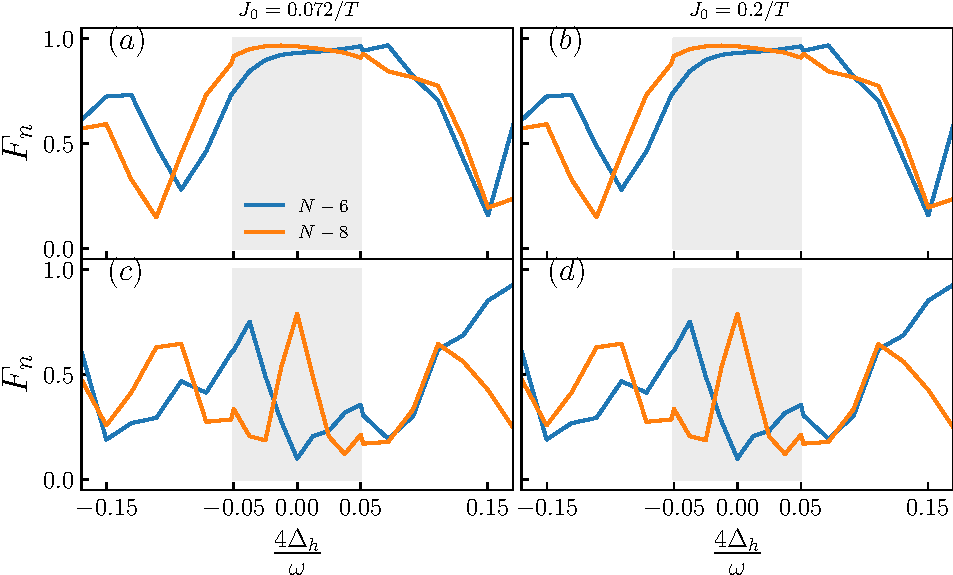
\includegraphics[width=10cm]{./figs/figure14.pdf}
				\end{center}
				\caption{Fidelity in relation to various deviation values, represented as $\frac{4\Delta_h}{\omega}$, for multiple system sizes (N) at 100T near the CDT/DL point under weak (panel a) and strong spin coupling conditions (panel b). With a steady drive frequency of $\omega= 20$, the amplitude deviation ($\Delta_h$) is incorporated into h. It's observed that the fidelity is significantly high near the CDT/DL point, which is indicated by a gray-colored area.}
				\label{Fig:aroundCDT}
			\end{figure}
		
			}
		\end{enumerate}
		
		\item The referee comments on, \comment{``\underline{DTC phase stability and entanglement entropy:}"}
		\begin{enumerate}
			\item \comment{``The paper seems to be intended for an audience from DTC and MBL/DMBL fields. However, for broader accessibility and comprehension, a brief introductory paragraph about realization and fundamental aspects of DTC within DMBL
			systems would be beneficial. How is DTC defined in these systems, and what are its fundamental properties? Additionally, how is $\omega$ chosen in relation to the periodicity of the Hamiltonian? Moreover, a preliminary explanation of how analyzing the time evolution of local magnetization and its FFT contributes to defining DTC would greatly enhance reader comprehension."}\\
			
			\response{ 
			We appreciate the referee's comment. We have added a concise introductory paragraph in the revised manuscript on page 3, which provides a general understanding of the DTC in DMBL systems. In this paragraph, we also discuss the definition of DTC and its fundamental properties.\\

			In order to stabilize a DTC in the system, previous studies included localization in the many-body system~\cite{Zhang2017, Zaletel2023}. In the proposed model we incorporate the localization by the dynamics of the system itself. In the earlier work we observed that DMBL is stable at higher frequencies~\cite{Mahbub2024}. Additionally, in this frequency limit we can apply Rotating Wave Approximation (RWA) which simplifies the analysis of systems with high-frequency driving fields. Thus, we have chosen $\omega=20$ for the numerical simulations. We have discussed this in the revised manuscript at section 3, page 7, last para.\\

			We have discussed how the time evolution of local magnetization and its FFT analysis contributes to detect DTC phase in the revised manuscript at page 3, para 2 and page 9, para 2.
			}\\

			\item \comment{``It is important to clarify the results shown in Fig. 7\footnote{Authors' note: Figure $7$ in the old manuscript has changed to Figure $9$ in the revised manuscript.}, where the behavior of regional magnetization might confuse new readers in the DTC field. This figure suggests that regional magnetization decreases over time under strong coupling and all-to-all interactions, which at the first glance seems to contradict the main text’s assertion that these conditions correspond to stable chimera states. Therefore, a comment  explaining how the magnetization relates to FFT based on the results would be helpful for correctly understanding the results."}\\
			
			\response{
			We thank the referee for the comment. We had stated in the earlier sections  that all-to-all interactions are the most suitable choice  for a stable chimera-like order as determined from relatively short-time simulations (around $80T$). We extended the simulations to longer times (around $2000T$) and updated the figure (figure 9 in the revised manuscript). The regional magnetization for all-to-all interaction and weak coupling  does not decrease appreciably even at these very large times. However, for strong couplings, appreciable beats are observed at these longer times. Running the other cases in the figure \sout{for longer times does not change the results significantly} \red{also exhibits melting in DTC phase accompanied with beats pattern}. We have included this discussion in the revised manuscript at page 18. 
			
			We have also analyzed the FFTs (amplitude-squares only) of the long-time $M^z_A$ data from the extended simulations. The dominant peak is at $\Omega=\omega/2$. However, there are smaller peaks in the neighborhood, corresponding to the beats seen in the time series data.
			For all-to-all interactions and weak coupling, the secondary peaks are unnoticeable. This manifests a stable chimera even at long times. However, for stronger coupling, the secondary peaks are larger. This indicates that the chimera-like order is less stable under strong coupling. We have included this discussion in the revised manuscript at page 18, para 2. 
			}
			\begin{figure}[h!]
				%\begin{center}
					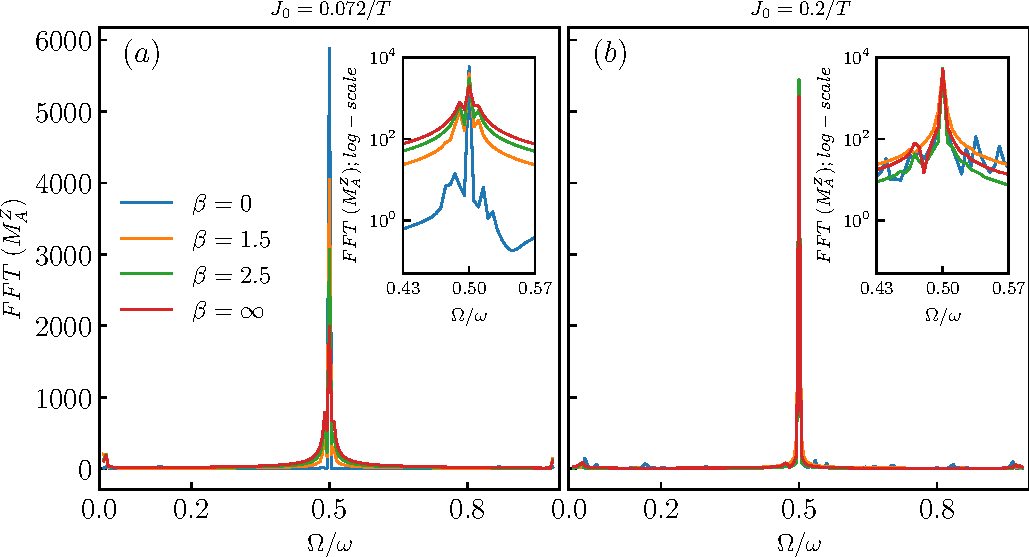
\includegraphics[width=10cm]{./figs/figure10.pdf}
				%\end{center}
				\caption{FFT for regonal magnetization ($M^z_A$) data obtained for time up to 2000T in region A. Weak(a-panel) and Strong (b-panel) is considered for several spin interaction ranges (defined by $\beta$) configuring the drive parameters at CDT/DL point. FFT is plotted also in log-scale plot in the inset of each panel for small frequency window to look closely into presence of frequencies is the temporal variation in $M^z_A$.}
				\label{Fig:regionalFFT}
			\end{figure}
			\item \comment{``There appears to be inconsistency in the analysis of EE and regional magnetisation along with FFT. EE is shown for almost two times longer dynamics that regional magnetization and FFT. Could the authors provide a comparison of regional  magnetization and its FFT for the extended time frames considered for entanglement entropy?"}\\
			
			\response{We thank the referee for pointing out our oversight. We have extended our numerical simulation for regional magnetization and corresponding FFT upto 2000T in order to keep consistency in analysis of EE and regional magnetization. We have updated figures(9) $\&$(10) in the revised manuscript.
			}
		\end{enumerate}
		\item The referee comments on, \comment{``\underline{Applications of chimera state:} The introduction of Section 4 briefly touches upon applications of chimera states, but it lacks depth. How can the chimera state findings be applied in practice? Expanding on potential applications and providing references to existing literature will be beneficial. This would enrich the discussion and highlight the practical relevance of their findings."}\\
		
		\response{Typically, an open quantum system is viewed as a Markov process where any information that is lost to the environment does not return to the system. However, in a chimera state, one part of the system can interact with an environmental system, while another part interacts with a non-Markovian environmental system. This means that information that is lost to the environment can potentially return to the system. Chimera states are therefore useful for studying these non-Markovian open systems.

		In addition, chimera states have potential applications in modern quantum devices. They can be used in NISQ (Noisy Intermediate Scale Quantum) processors to distinguish between the relatively clean and noisy qubits. Normally, information diffusion starts with the noisy qubits, leading to the quantum state slowly decohering into a classical mixed state. But by using a chimera state, the clean qubits can be shielded, effectively extending the coherence time. This enables more sophisticated quantum information processing.}\todo[inline]{Application part, written by Akitada. Please review.}
	\end{enumerate}

	\item[] {\bf Minor Comments}
	\begin{enumerate}
		\item The referee says, \comment{``\underline{Page 6, lines 30-31 and page 18, lines 47-48:} please add a reference to the Baker-Campbell-Hausdorff formula, e.g. [67] as in the Appendix B, page 22, lines 44-45"}\\
		
		\response{We regret the oversight and thank the referee for raising this issue. In the revised manuscript, we have included the seminal reference to the BKH formula at the indicated spot.}
		\item The referee says, \comment{``\underline{Page 6, lines 46-48:} clarify what is $\mathcal{J}_0$, e.g. “of the higher roots of zeroth-order Bessel function $\mathcal{J}_0$”"}\\
		
		\response{We thank the referee for the comment. As we have indicated earlier, any root of Bessel function $\mathcal{J}_0\left(\frac{4h}{\omega}\right)$ is sufficient to dynamically localize the dynamics of $\hat{H}_2$. We have updated the manuscript by removing the word "higher", hopefully eliminating any confusion.
		\item The referee comments on, \comment{``\underline{Page 8, caption of Fig. 3:}"}}
		\begin{enumerate}
			\item The referee says, \comment{``refine the caption for clarity: “plotted for different values of amplitude h of the periodic drive. The x-coordinate plots 4h/$\omega$, where drive frequency is kept constant $\omega$=20..."}\\
			
			\response{We thank the referee for the comment. We have modified the sentence in the revised manuscript to ``The quasi-energies are plotted against $4h/\omega$, where the drive frequency $\omega=20$ is fixed, and drive amplitude $h$ is vatried." in order to maintain clarity in content in manuscript.}\\
			
			\item The referee says, \comment{``The first such point is shown...” $\rightarrow$ “The first two points are shown..."}
			
			\response{We thank the referee for the comment and suggestion. We have modified the sentence in the revised manuscript accordingly.}
		\end{enumerate}
	
		\item The referee comments on, \comment{``\underline{Page 9, caption of Fig. 4:}"}
		\begin{enumerate}
			\item The referee says, \comment{``This is the suggestion of a notation change for smoother reading: “Site(i)” → “i”, 
			e.g. “for each i-th spin at region A (i=0,1,2,3) and region B (i=4,5,6,7)...”. To implement this modification consistently: change the x-coordinate labels in the Fig. 4 from “Site(i)” → “i”, and update accordingly the main text/ figures/ captions to
			maintain consistency"}\\
		
			\response{We thank the referee for the suggestion. We have modified the caption and figures by replacing ``Site(i)” → ``i” through out the manuscript.}
			\item The referee says, \comment{``Revise “spin coupling ($J_0$=0.027/T)” $\rightarrow$ “spin coupling ($J_0$=0.072/T)”}\\
			
			\response{We thank the referee for pointing out the typographical error. We have corrected it to ``($J_0$=0.072/T)" in the revised manuscript.}\\
			\item The referee says, \comment{``Please add also the information for which root of the Bessel function the plot is obtained."}\\
			
			\response{We thank the referee for the comment. As explained earlier, we had defaulted to the first root of Bessel function for all numerical simulations, choosing higher roots for a few selected cases. We have corrected them all to the first root in the revised manuscript and updated the caption of figure 4 accordingly.}\\
		\end{enumerate}
		\item The referee comments on, \comment{``\underline{Page 10, Fig. 5:}"}
		\begin{enumerate}
			\item The referee says, \comment{``Define $M_A^z$, which appears in the y-label, in the main text or the caption for
			clarity. The formal introduction of regional magnetization occurs in Section 4, while Fig. 5 is situated within Section 3."}\\
			\todo[inline]{Review from here.}
			\response{We appreciate the referee for bringing our oversight to our attention. The labelling of y-coordinate ``$FFT(M^Z_A)$'' was incorrect in figure 5 in earlier manuscript. The figure was actually meant to represent the FFT analysis of the local magnetization $\expval{\hat{S_z^i}}$ at a specific site $i=1$ in region A. We have now rectified and updated the figure in the revised manuscript.}\\
			
			\item The referee says, \comment{``Specify a CDT/DL point, i.e. to which root of the Bessel function it corresponds"}\\
			
			\response{We thank the referee for the comment. We had defaulted to the first root of Bessel function for all numerical simulations and we have this selection of CDT/DL point consistently thorughout in the revised manuscript.}\\
		\end{enumerate}
		\item The referee comments on, \comment{``\underline{Page 11, lines 50-51:} Specify “a CDT/DL point...” while throughout the paper the root of the Bessel function is changing, e.g. Fig. 4 and Fig. 5"}\\
		
		\response{We thank the referee for the comment. We have defaulted the first root of $\mathcal{J}_0\left(\frac{4h}{\omega}\right)$ as the CDT/DL point and we have this selection of CDT/DL point consistently thorughout the revised manuscript.}\\
		
		\item The referee comments on, \comment{``\underline{Page 13, Fig 8:} Correct the notation “$\omega/\omega_D$” → “$\Omega/\omega$”"}\\
		
		\response{We thank the referee to point out the typographical error. We have corrected “$\omega/\omega_D$” → “$\Omega/\omega$” in the caption of the respective figure the revised manuscript.}\\
		\item The referee says, \comment{``Ensure all paper captions are reviewed for consistency. Additionally, include all relevant
			parameters in the captions that would enable interested readers to reproduce your
			results effectively."}\\
		
		\response{We thank the referee for the comment and kind suggestion. We have gone through the entire manuscript and maintained consistency in the parameters and notations. We expect  better comprehension and feasibility in reproduction of all the findings we present in this paper.}
	\end{enumerate}

	\newpage
	\noindent \textbf{Response to the Referee: 3's comment}
	\begin{enumerate}
		\item The referee says, \comment{``My main concern is regarding the context in which the word “chimera” has been used
			in this work. The word chimera was originally used for the co-existence of synchronized and unsynchronized dynamics of coupled “identical” oscillators in the “Phys. Rev. Lett. 93, 174102 (2004)” which was initially discovered in the following
			works “Y. Kuramoto and D. Battogtokh, Nonlinear Phenom. Complex Syst. 5, 380 (2002), S. I. Shima and Y. Kuramoto, Phys. Rev. E 69, 036213 (2004)”. The surprise that led to the discovery of the chimera state resided in the fact that all the
			subsystems were identical and were subjected to the same environment but behaved differently only due to different initial configurations. But in this and the earlier work mentioned by authors “Phys. Rev. Lett. 126, 120606 (2021)”, regions A and B are under different drive conditions. Hence, the spins in these regions are not under identical environments. In such a configuration, it is trivial that both regions can behave differently since they are subjected to different drive conditions. Hence, this co-existence of different phases under inhomogeneous drive conditions for different
			regions does not fall under the novel phenomenon of “chimera”.\\
			
			I understand that this issue arises due to the fact that the related work “Phys. Rev. Lett. 126, 120606 (2021)” has referred to this phenomenon as a “chimera state”, even though one of the authors from the same paper has used the definition of the identical oscillator in their earlier work “Phys. Rev. E 92, 062924 (2015)”. Therefore, I request the authors either remove the word chimera completely or use the word “chimeralike state” which has been used in the work “Phys. Rev. E 103, 012214 (2021)” where authors have discovered a chimeralike state in almost-identical oscillators. Along with this, authors should provide a clear distinction that the definition of “chimeralike state” used in this work differs from the definition involving identical oscillators and follows from the earlier work “Phys. Rev. Lett. 126, 120606 (2021)” and “Phys. Rev. E 103, 012214” which involve non-identical systems. I
			suppose this is crucial to avoid misunderstandings and further confusion about the novel “Chimera State” for the readers of this reputed journal."}\\
		
			\response{We value the referee's critique and suggestion. We concur with the referee that the quantum spin-1/2 chimera state differs from the classical chimera in identical oscillator systems. Our proposed quantum model includes two non-homogeneous Hamiltonians, which contradicts the classical chimera phenomenon's requirement of identical oscillators in similar environments. This is more akin to the nonlocally coupled system in classical systems that resemble chimeras~\cite{Sharma2021}. Quantum mechanics employs linear Schrödinger dynamics, in contrast to the potential non-linearity of classical dynamics. Therefore, emergent phenomena in quantum mechanics are not directly comparable to classical occurrences. This brings into question the appropriateness of naming a new phenomenon a "chimera" in our proposed quantum system. We are grateful for the referee's suggestion to replace the term "chimera state" with "chimeralike state." In accordance with the referee's advice, we have replaced all instances of 'chimera state' with 'chimeralike state' and 'chimera order' with 'chimeralike order' in the revised manuscript and title.}\\
		
		\item The referee says, \comment{``Adding to the previous point on chimera-like states, it would be interesting to see if the chimera state emerges even for almost the same drive conditions for regions A and B, i.e. for $\epsilon A \approx \epsilon B$ where they only differ by a small value."}\\	
			
		\response{	
		We appreciate the comment provided by the referee. We have expanded our study to include conditions where the spin rotational errors $\epsilon_{A,B}$ are in close proximity, specifically when $\epsilon_A \approx \epsilon_B$. In the revised manuscript, we have included a figure (Figure 8. page 16) that showcases the regional magnetization values at different panels we obtained through numerical calculations. We ensured that $\epsilon_A \approx \epsilon_B$ for various spin interaction ranges. We observed that when $\epsilon_A$ and $\epsilon_B$ both are small (panel-g ), the spins in both region A and B display time crystalline behavior. However, over time, the DTC phase eventually dissolves. As the values of $\epsilon_A$ and $\epsilon_B$ gradually increase, we observe the gradual emergence of the DMBL phase in both regions and when $\epsilon_A$ and $\epsilon_B$ are both large we observe DMBL in either  the regions A and B (panel-h). Therefore, it is not possible for a stable DTC-DMBL chimeralike order to occur when the values of $\epsilon_A$ and $\epsilon_B$ are approximately equal. We have introduced this discussion in the revised manuscript at section 5.1, para 2 on page 15.
		}\\
	
		\item The referee says, \comment{``Authors can also investigate the onset of the chimera state as a function of $\epsilon A$ - $\epsilon B$."}\\
		
		\response{We thank the referee for the comment. We have considered a large set of $\epsilon_A$ and $\epsilon_B$ in order to investigate the dependence of stability of the DTC-DMBL chimeralike order and numerically calculated regional magnetization and plotted in figure 8. In the figure we have considered a small value of $\epsilon_A$ and then varied $\epsilon_B$ and vice versa. We observe that when $\epsilon_A$ - $\epsilon_B$ is minimum $~\sim -1.0$ the DTC in region A and DMBL in region B is most stable as can be observed in panel-(a) in figure 8. It is intriguing that when   $\epsilon_A$ - $\epsilon_B$ is maximum $~\sim +1.0$ a stable DTC can be found in region B and a subtle DMBL is found in region A. This concluded that at the extremum values of  $\epsilon_A$ - $\epsilon_B$, a stable DTC-DMBL chimera like order occurs. Also varying $\epsilon_A$ - $\epsilon_B$ values regional selection over phases can be controlled. We have discussed it in revised manuscript from page 13 to 15, section 5.1 Regional magnetization. }
		
		\item The referee says, \comment{``To avoid confusion, the 45th line of Page 2 should be modified to indicate that the concept of “time crystal” was introduced by Frank Wilczek, not just the Discrete time crystals."}\\
		
		\response{We thank the referee for pointing out the mistake. We have corrected and modified the sentence from `` The concept was
		first proposed by Frank Wilczek " to ``The time crystal (TC) was first proposed by Frank Wilczek \dots" in the revised manuscript.}
	
		\item The referee says, \comment{``$J_0$ is not defined after equation 7 in the main text."}\\
		
		\response{We thank the referee for pointing out the typographical error. We have replaced $\mathcal{J}_0$ with $\mathcal{J}_0\left(\frac{4h}{\omega}\right)$. in the revised manuscript.}
		
		\item The referee says, \comment{``Recent works have not been included in the manuscript, I list some of the recent work on chimera states in time crystals and observation of discrete-time crystals for the consideration of authors:."}
		\begin{enumerate}
			\item \comment{``Observation of a Dissipative Time Crystal”, Phys. Rev. Lett. 127, 043602 (2021)"}
			\item \comment{``Observation of a Prethermal U(1) Discrete Time Crystal”, Phys. Rev. X 13, 041016 (2023)"}
			\item \comment{``Observation of time crystal comb in a driven-dissipative system”, arXiv:2402.13112 (2024)}
			\item \comment{``Exotic synchronization in continuous time crystals outside the symmetric subspace”, arXiv:2401.00675 (2024)"}\\
		\end{enumerate}
		
		\response{
		We thank the referee for the suggestion. We have included the recent works suggested by the referee in the introduction section in para 3 on page 2. 
		}\\
	\end{enumerate}
\end{enumerate}
		
\noindent \textbf{Summary of important changes to the  manuscript}
\begin{enumerate}
	\item write the changes you have made$\dots$.
\end{enumerate}

%Bibliography
\bibliography{dtcdmbl.bib}
\bibliographystyle{apsrev4-2}

\end{document}